\begin{figure*}[!t]
  \centering
  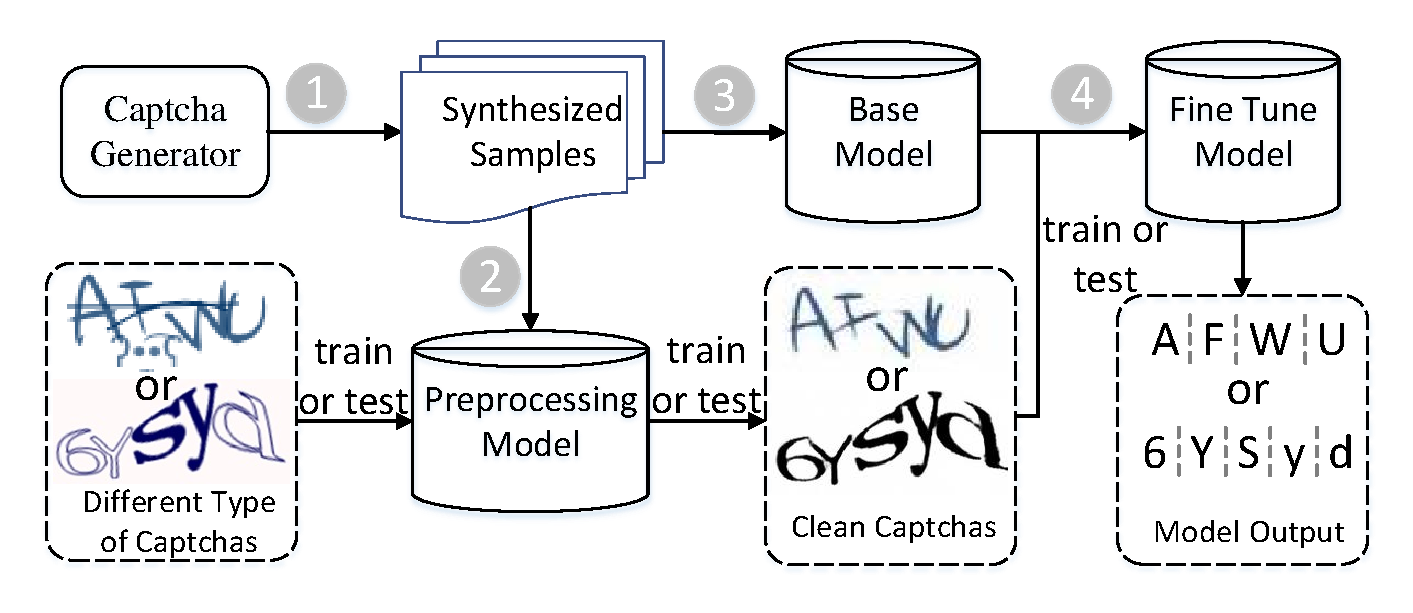
\includegraphics[width=0.8\textwidth]{fig/overview/overview.pdf}
  \caption{The overview of our attack.}
  \label{fig:overview}
\end{figure*}

\section{Background}
\subsection{Security Features of Text-based Captchas \label{section: security_features}}
Recent text-based captchas have employed a range of security features to withstand automated solving. These features include negative
kerning (also known as character collapsing), distortion, occluding lines, noise background etc.

To summary out a representative security features, we collected a wide range of real captchas that had ever been or being used by the top 50 most popular websites listed by Alexa~\footnote{http://www.alexa.com/topsites}. Figure~\ref{fig:text-based captchas} gives some representative examples of our collected Captchas~\footnote{Some previous used Captchas come from the related works~\cite{Gao2013The,Gao2016A,Bursztein2011Text}.}.
The security features can be classified into two categories: anti-segmentation feature and anti-recognition feature. The anti-segmentation feature aims to increase the difficulty of character segmentation, and it includes connection lines, character overlapping and noise background as shown in Figure~\ref{fig:security_features} (1), (2), (6). 
The anti-recognition feature can defense against recognizing by changing the font style of part characters and it consists of different font sizes and colors, solid and hollow font and character rotating, distortion and waving as shown in Figure~\ref{fig:security_features} (3), (4), (5).

\begin{figure}[!t]
  \centering
  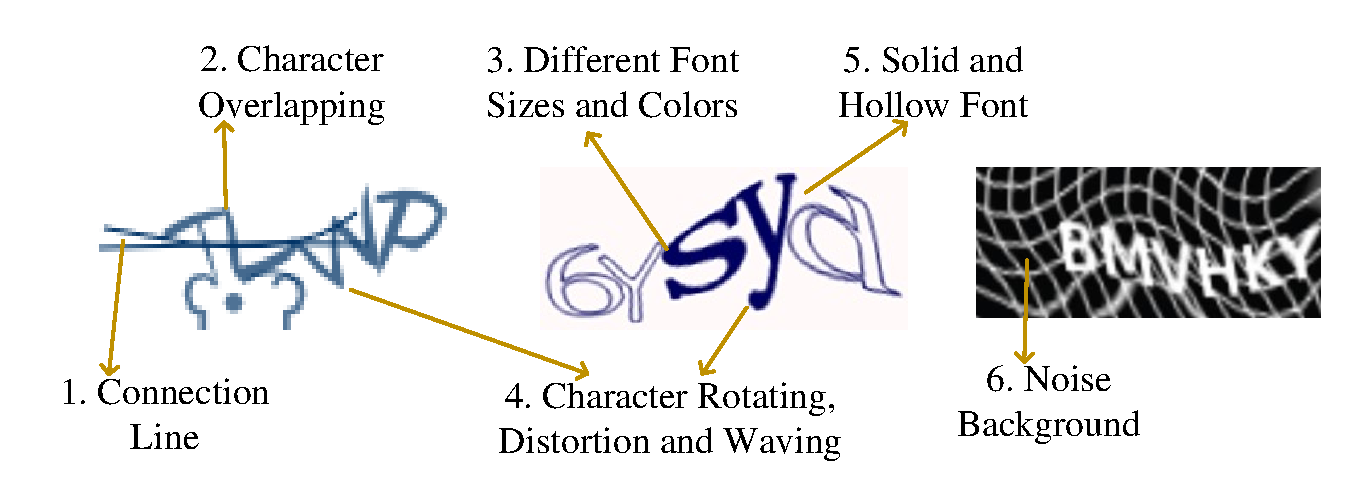
\includegraphics[width=0.45\textwidth]{fig/security_features/security_features.pdf}
  \caption{The security features of captchas.}
  \label{fig:security_features}
\end{figure}
 %To do so, the captcha is comprised of overlapping characters and is improved by sophisticated noise background and extra connection lines. Thus, the anti-segmentation feature is the global feature because it makes the whole captcha complex.
%In contrary, the anti-recognition feature belongs to local feature. It can defense against automated recognizing characters by changing the font style of part characters. We list the two features in details below.

%\noindent \textbf{Anti-segmentation features} \textbf{1. Noise Background:} Try to make the background color that has little difference with the text for confusing the solver. \textbf{2. Connection Lines:} Add extra line segments on the text to prevent solver from automatic finding the single character. \textbf{3. Overlapping} Decreasing the space between the adjacent characters to make them collapsed.
%
%\noindent \textbf{Anti-recognition features} \textbf{1. Character Set:} Which charset the text-based Captcha scheme uses. Some schemes only include English letters while some schemes consist of both English letters and Arabic numerals. \textbf{2. Font Style:} Using multiple font styles such as solid font, hollow font or font comprised of dots. \textbf{3. Font Size} Using random font size when generating captchas. \textbf{4. Font Color:} Using variable font colors. \textbf{5. Distortion:} Distorting characters using attractor fields. \textbf{6. Rotating:} Rotating characters with random angles. \textbf{7. Waving:} Distorting the characters in a wave fashion.
%
%\FIXME{TODO: Will come to this later. We need to cut the crap in text.}

\subsection{Generative Adversarial Networks}
Our approach is inspired by the recent breakthrough of effectiveness of generative adversarial networks
(\GANs)~\cite{Goodfellow2014Generative}. A \GAN consists of two models: a generative model for creating synthesized examples and a
discriminative model to distinguish the synthesized examples from the real ones. Backpropagation is applied to train both models so that
the generator produces better synthesized samples, while the discriminator becomes more skilled at flagging synthetic samples. \GANs have
shown impressive results in image ~\cite{pix2pix2016,CycleGAN2017} and natural language processing~\cite{Yu2016SeqGAN,Li2017Adversarial}.
However, due to the newness of the technique, no work so far has exploited \GANs to develop a generic approach to attack text-based
captchas.

%\subsection{Text-based Captchas}
%
%CAPTCHA is also called inverse Turing test~\cite{Naor1996Verification}, and aims to determine whether or not the user is human. The most popularity of Captchas is text-based Captchas. Initially, they were composed of deformed English letters and Arabic numerals which human can recognize while computers cannot. The usage of English letters and Arabic numerals makes text-based Captchas being welcomed world-wide~\cite{Chellapilla2005Building,Chellapilla2005Computers}. Due to such advantages, text-bsaed Captchas have been widely used in various of Internet security access tasks~\cite{Von2004Telling}. These tasks include defending against malicious scraping web contents, preventing automatic registration of free accounts for spam posting or forums, or mitigating the impact of DDoS attacks.
%
%\subsubsection{Captcha Security Features} \label{section: sccturity_features}
%To summary out a representative security features, we collected a wide range of Captchas that had ever been or being used by the top 50 most popular web sites which are listed by Alexa~\footnote{http://www.alexa.com/topsites}. Figure~\ref{fig:text-based captchas} gives some representative examples of our collected Captchas~\footnote{Some previous used Captchas come from the related works~\cite{Gao2013The,Gao2016A,Bursztein2011Text}.}. It obviously shows that current text-based Captchas have more complex security features than previous Captchas. These features can be classified into two categories: anti-segmentation and anti-recognition features.
%The anti-segmentation feature aims to increase the difficulty of character segmentation. In order to implement such feature, the Captcha is needed to be confused on the whole with sophisticated background, extra connecting lines and overlapping characters. Thus, the anti-segmentation features can be regarded as the global security features as it makes the Captcha complex on the whole.
%In contrary, the anti-recognition features belong to local features. It can defense against automated recognizing characters by changing the font style of characters.
%We list the two fratures as follows:
%
%\noindent \textbf{Anti-segmentation features} \textbf{1. Sophisticated Noisy Background} Try to make the background have little difference with the text for confusing the solver. \textbf{2. Connection Lines} Add extra lines on the text to prevent solver from automatic finding the single character.
%\textbf{3. Overlapping} Decreasing the space between the adjacent characters to make them collapsed.
%
%\noindent \textbf{Anti-recognition features} \textbf{1. Character Set} Which charset the text-based Captchas scheme uses. Some schemes only include English letters while some schemes consist of both English letters and Arabic numerals. \textbf{2. Font Style} Using multiple font styles such as solid font, hollow font or font compromise of dots. \textbf{3. Font Size} Using random font size when generating Captcha. \textbf{4. Font Color} Using variable font colors. \textbf{5. Distortion} Distorting characters using attractor fields. \textbf{6. Rotating} Rotating characters with random angles. \textbf{7. Waving} Distorting the characters in a wave fashion.
%
%\subsubsection{Previous Captcha Scheme}
%According to the~\cite{Gao2016A}, the previous text-based Captchas can be classified into three categories: character isolated Captcha (Figure~\ref{fig:text-based captchas} (a)), hollow character Captcha (Figure~\ref{fig:text-based captchas} (c)) and Connecting Characters Together (CCT) Captcha (Figure~\ref{fig:text-based captchas} (b) and (d)) based on font style and the space between adjacent characters. Obviously, most of previous text-based Captchas use a single anti-segmentation or anti-recognition features. For examples, Figure~\ref{fig:text-based captchas} (a) only uses one single anti-recognition feature (slight rotating) and Figure~\ref{fig:text-based captchas} (b) uses one anti-segmentation feature (character overlapping) and one anti-recognition feature (character waving).
%Of course, some Captcha schemes use a simple combination of the above security features such as Figure~\ref{fig:text-based captchas} (f) uses rotating, background and connection lines. Although using multiple anti-segmentation and anti-recognition features, the text have the same font style or obvious difference comparing to the background.
%
%Thus, the robustness of text-based Captchas is an active topic in the research communities. Researchers have comprehensively evaluated the security of text-based Captchas~\cite{Bursztein2011Text,Bursztein2014The,Gao2016A}.
%They demonstrate that text-based Captchas are vulnerable under their attacks as they are able to effectively segment each character. Although the security of text-based Captcha scheme are suspicious by research communities, such scheme is still primary authentication mechanism and are widely deployed most mainstream websites. This wide-spread usage, we think, is due to the following reasons:
%(1) the written text on Captcha image may be presented in many styles such as distorted, rotated, hollow, or overlapping characters, complex noisy background or noise interference.
%Each of these styles can be designed more complex than previous. For examples, the value of character's rotating angle can be set more larger than previous, and the background can be became more complex.
%(2) The conbination of these styles is able to increase the security strength of Captchas so that it can defeat against current attacks. Current Captchas (Figure~\ref{fig:text-based captchas} (2)) combine many anti-segmentation and anti-recognition features than previous Captchas (See Figure~\ref{fig:text-based captchas} (1)). This increases the security of text-based Captchas. Recent studies suggests that text-based Captchas are still a security mechanism if they are properly designed~\cite{Thomas2013Trafficking,Bursztein2014Easy}. In the following, we will introduce the current Captcha scheme.
%
%\begin{table*}[t]
%    \centering
%    \caption{Mappings from security features to its corresponding numbers}
%    \scriptsize
%    \label{table: feature_number}
%    \begin{tabular}{l|ccc|ccccccc}
%        \toprule
%        & \multicolumn{3}{|c|}{\textbf{Anti-segmentation Features}} & \multicolumn{7}{|c}{\textbf{Anti-recognition Features}} \\
%        \multirow{-2}{*}{\textbf{Security Features}} & Background & Connection Lines & Overlapping & Char Set & Font Style & Font Size & Font Color & Distortion & Rotating & Waving \\
%        \midrule
%        \textbf{Feature Number} & \circled{0} & \circled{1} & \circled{2} & \circled{3} & \circled{4} & \circled{5} & \circled{6} & \circled{7} & \circled{8} & \circled{9} \\
%        \midrule
%        \textbf{Param Value} & Fixed or Random & \tabincell{c}{Number, \\ Location} & \tabincell{c}{Fixed or \\ Random} & \multicolumn{7}{c}{Fixed or Random} \\
%        \bottomrule
%    \end{tabular}
%\end{table*}
%
%\subsubsection{Current Captcha Scheme}
%Current Captcha scheme combines many anti-segmentation and anti-recognition features. This makes current text-based Captchas more complex than previous Captcha schemes. Figure~\ref{fig:text-based captchas} (2) shows some representative current Captcha schemes. Obviously, it presents that each current Captcha scheme is compromised of many security features such as different font style, character overlapping, rotating and distorting, connecting lines and so on. Take Figure~\ref{fig:text-based captchas} (k) for an example, this Captcha using two anti-segmentation features (complex background and connecting lines) and five anti-recognition features (Character Set: both English letters and Arabic numerals, Font Style: both solid font and hollow font, Font Size: different font size, Font Color: different font color, Rotating: rotating character with different angles.). Likewise, other Captchas presented in Figure~\ref{fig:text-based captchas} also uses many anti-segmentation and anti-recognition features.
%
%Previous attacking methods on Captchas cannot directly crack current complex text-based Captchas.
%The pixel counting approach proposed by Yan \emph{et al.}~\cite{Yan2007Breaking} will lose their efficiency in current Captchas. This is because the character sizes of current Captchas are different, which leads to the number of pixels is not fixed.
%Color Filling Segmentation (CFS) method proposed by Yan and used by Gao~\cite{Yan2008A,Gao2013The} are also cast into the shade as sometimes the characters on current Captcha are overlapped, and CFS method cannot segment the connected character.
%The powerful generic attacks which claim to crack a wide range of text-based Captchas have been proposed~\cite{Bursztein2014The,Gao2016A}. The attack described in~\cite{Bursztein2014The} is a state-of-the-art way to segment the characters. However, this approach cannot effectively segment the characters when the space between adjacent characters is -3 pixel which is more than the space (generally about -4 pixel) between the adjacent characters of current Captcha.
%The work in~\cite{Gao2016A} exploits Gabor filters to extract character components, and then rank the adjacent character components to recombine the individual characters. The major issue of this method is the high error ranking rate whiling cracking hollow characters. This is because the hollow characters will be extracted many possible tiny components, which results in many candidate combinations, increasing the error rate.
%Thus, comparing to previous Captchas, current Captcha scheme deployed by many popular web sites are more robustness, and can defeat against previous attacks.
%
%In terms of the above complex Captcha schemes, this paper presents a hierarchical attack method using deep learning technology.
%Our approach is able to dynamic adapt the different styles of Captchas. Specifically, to the Captchas with confusing background, our method can effectively clean up the complex background. To the Captchas with overlapping characters, our method can expand the space between adjacent characters. To the Captchas with both cases, our method first remove the background and then enlarge the space of adjacent characters.
%%Unlike previous attacks, our method is able to effectively clean up the complex background and connecting lines, and then the space between adjacent overlapping characters can be expanded as much as possible. At last, we explore to translate the distorted character to a regular one for the purpose of improve the success rate using CNN recognition engine.
%Our work aims to call the community to revisit the security of text-based Captchas under the age of Artificial Intelligence.
%
%\subsection{Generative Adversarial Networks} \label{section: GANs}
%
%Generative Adversarial Networks (GANs) is a special type of Artificial Neural Network (ANN), and it was first proposed by Goodfellow in 2014~\cite{Goodfellow2014Generative}. GANs consists of two neural networks competing with each other: one is the generative model \emph{G} that generates the data which similar to the true data; the other is the discriminative model \emph{D} which validate whether the inputting data comes from the training data or \emph{G}. By repeating this competing procedure iteratively, this game will be terminated if the discriminative model \emph{D} cannot identify the inputting data comes from training data or the generative model \emph{G}.
%
%The adversarial trait of GANs makes it has been widely used in video predicting~\cite{Walker2017The}, image processing~\cite{pix2pix2016,CycleGAN2017}, natural language processing~\cite{Yu2016SeqGAN,Li2017Adversarial}, code security~\cite{Xu2016Automatically,Liu2016Delving}. Among these fine studies, Phillip \emph{et al.}~\cite{pix2pix2016} proposed an image-to-image translation method named \emph{Pix2Pix}~\cite{Pix2PixCode} using the conditional GANs\footnote{Conditional GANs learn a mapping from observed image with random noise to output image while GANs learn the mapping from only random noise to output image.} (cGANs)~\cite{Mirza2014Conditional}.
%In their work, they can translate an image from one style to another.
%Differ from typical GANs, cGANs consists of conditional generator and discriminator. Both the conditional generator and discriminator take the observed image as an input image so that cGANs can converge to a stable state.
%
%This work inspired us that can it translate the hardly recognizing Captchas to easy identifying one?
%That is can we effectively remove the confusing background, expand the space of adjacent characters or mitigate the deformed characters?
%To do this, we design an effectively segment and recognize method for Captchas using a variant of \emph{Pix2Pix}~\cite{Pix2PixCode}.
%Our method is able to clean up the complex background and connecting lines on Captcha image, expand the space between the adjacent characters and translate the distorted character to the regular one.
%The preliminary experiments prove this method is valid. To our best knowledge, this is the first work to attack Captchas using GANs.
